\section{Proofs for the Main-Text Guarantees}
\label{app:theory}

The guarantees in Section~\ref{sec:method} justify source-coordinate estimation and stability with respect to coordinate error only. They do not establish low-dimensionality, semantic sufficiency, task identifiability, or cross-task relational generalisation.

\subsection{Proof of Proposition~\ref{prop:source-concentration}}

Let $Y_i=h_\psi(X_i)-\mu$. Then $\E[Y_i]=0$, the $Y_i$ are independent, and
\[
\bar h_M-\mu=\frac{1}{M}\sum_{i=1}^{M}Y_i.
\]
By the $L_\rho$-Lipschitz property of $\rho_\psi$,
\[
\|z_M-\rho_\psi(\mu)\|_2^2
\leq
L_\rho^2\|\bar h_M-\mu\|_2^2.
\]
Taking expectations and expanding,
\begin{align*}
\E\|\bar h_M-\mu\|_2^2
&=
\frac{1}{M^2}
\E\left\|\sum_{i=1}^{M}Y_i\right\|_2^2\\
&=
\frac{1}{M^2}
\left[
\sum_{i=1}^{M}\E\|Y_i\|_2^2
+
2\sum_{i<j}\E\langle Y_i,Y_j\rangle
\right].
\end{align*}
For $i\neq j$, independence and zero mean imply
\[
\E\langle Y_i,Y_j\rangle
=
\langle \E Y_i,\E Y_j\rangle=0.
\]
Hence
\[
\E\|\bar h_M-\mu\|_2^2
=
\frac{1}{M}\E\|h_\psi(X)-\mu\|_2^2
=
\frac{\mathrm{tr}(\mathrm{Cov}[h_\psi(X)])}{M}.
\]
Combining the last two displays yields
\[
\E\|z_M-\rho_\psi(\mu)\|_2^2
\leq
\frac{L_\rho^2\,\mathrm{tr}(\mathrm{Cov}[h_\psi(X)])}{M}.
\]
This proves Proposition~\ref{prop:source-concentration}. The result controls estimation variance around the population feature coordinate; it does not imply that this coordinate is semantically sufficient.

\subsection{Proof of Proposition~\ref{prop:coordinate-stability}}

Let $X_t^z$ and $X_t^{z'}$ solve the reverse SDE with the same initial random variable and the same Brownian path, and write
\[
\Delta_t=X_t^z-X_t^{z'}.
\]
Because the diffusion coefficient does not depend on $z$, the stochastic increments cancel under this synchronous coupling. With $\Delta_0=0$,
\[
\Delta_t
=
\int_0^t
\bigl[
b_z(X_s^z,s)-b_{z'}(X_s^{z'},s)
\bigr]\,ds.
\]
Adding and subtracting $b_z(X_s^{z'},s)$ gives
\begin{align*}
\|\Delta_t\|_2
&\leq
\int_0^t
\|b_z(X_s^z,s)-b_z(X_s^{z'},s)\|_2\,ds\\
&\quad+
\int_0^t
\|b_z(X_s^{z'},s)-b_{z'}(X_s^{z'},s)\|_2\,ds.
\end{align*}
The state-Lipschitz assumption bounds the first integrand by $L_x\|\Delta_s\|_2$. For the second,
\[
b_z(x,s)-b_{z'}(x,s)
=
-g(s)^2B(x,s)(z-z'),
\]
so
\[
\|b_z(x,s)-b_{z'}(x,s)\|_2
\leq
L_z\|z-z'\|_2.
\]
Therefore
\[
\|\Delta_t\|_2
\leq
L_x\int_0^t\|\Delta_s\|_2\,ds
+
L_z t\|z-z'\|_2.
\]
The integral form of Gr\"onwall's inequality yields
\[
\|\Delta_t\|_2
\leq
L_z\|z-z'\|_2
\int_0^t e^{L_x(t-s)}\,ds
=
L_z\phi_{L_x}(t)\|z-z'\|_2,
\]
where
\[
\phi_{L_x}(t)=
\begin{cases}
(e^{L_xt}-1)/L_x,&L_x>0,\\
t,&L_x=0.
\end{cases}
\]
Since $\phi_{L_x}$ is nondecreasing,
\[
\sup_{t\leq T}\|\Delta_t\|_2
\leq
L_z\phi_{L_x}(T)\|z-z'\|_2.
\]
Squaring and taking expectations proves the first claim with
$C_T=L_z^2\phi_{L_x}(T)^2$.

For the Wasserstein statement, the synchronous construction is a valid coupling of the endpoint laws $P_z$ and $P_{z'}$. Hence
\[
W_2(P_z,P_{z'})^2
\leq
\E\|X_T^z-X_T^{z'}\|_2^2
\leq
C_T\|z-z'\|_2^2,
\]
and taking square roots completes the proof.

The proposition establishes continuity of the generated law with respect to $z$ under the stated regularity assumptions. It does not imply that the learned coordinate is low-dimensional, task-identifying, or transferable across unseen semantic tasks.

\FloatBarrier

\section{Gaussian-Mixture Experiments}
\label{app:gmm}

\subsection{Coordinate calibration}
Five separate 2-D Gaussian-mixture families check whether the learned generator responds to task coordinates. We evaluate calibration on each corresponding 80k-step checkpoint using 32 held-out tasks, $K_T=5$ and eight noise draws per task. The mean-minus-own loss interval is positive in 5 of the five families. These conditioning diagnostics remain separate from the factorial boundary study.

\begin{table}[h]
\centering\small
\caption{GMM calibration on five separate 80k-step checkpoints. Each uses 32 held-out tasks; eight noise draws are averaged within task. $\Delta_{\rm task}=L(\bar z)-L(z_y)$ has a paired task-level 95\% half-width. This is a coordinate intervention, not a deployment comparison.}
\begin{tabular}{lccc}
\toprule
Task family & Own & Mean & $\Delta_{\rm task}$\\
\midrule
Perturbation .10 & $0.4398$ & $0.5956$ & $0.1558\pm0.0286\sigstar$\\
Perturbation .25 & $0.4912$ & $0.6125$ & $0.1212\pm0.0232\sigstar$\\
Perturbation .50 & $0.5847$ & $0.6729$ & $0.0882\pm0.0272\sigstar$\\
Perturbation 1.00 & $0.6684$ & $0.7591$ & $0.0907\pm0.0423\sigstar$\\
Unrelated & $0.5427$ & $0.6386$ & $0.0959\pm0.0341\sigstar$\\
\bottomrule
\end{tabular}
\end{table}

Figure~\ref{fig:coord-profile} has two different checkpoint sources: the GMM panel uses the 80k-step perturbation-0.1 checkpoint, and the CIFAR panel uses the 50k-step \texttt{cifar\_ds3} checkpoint. They interpolate encoder coordinates and diagnose conditioning; neither panel directly measures correct-source deployment superiority.

\begin{figure}[t]
\centering
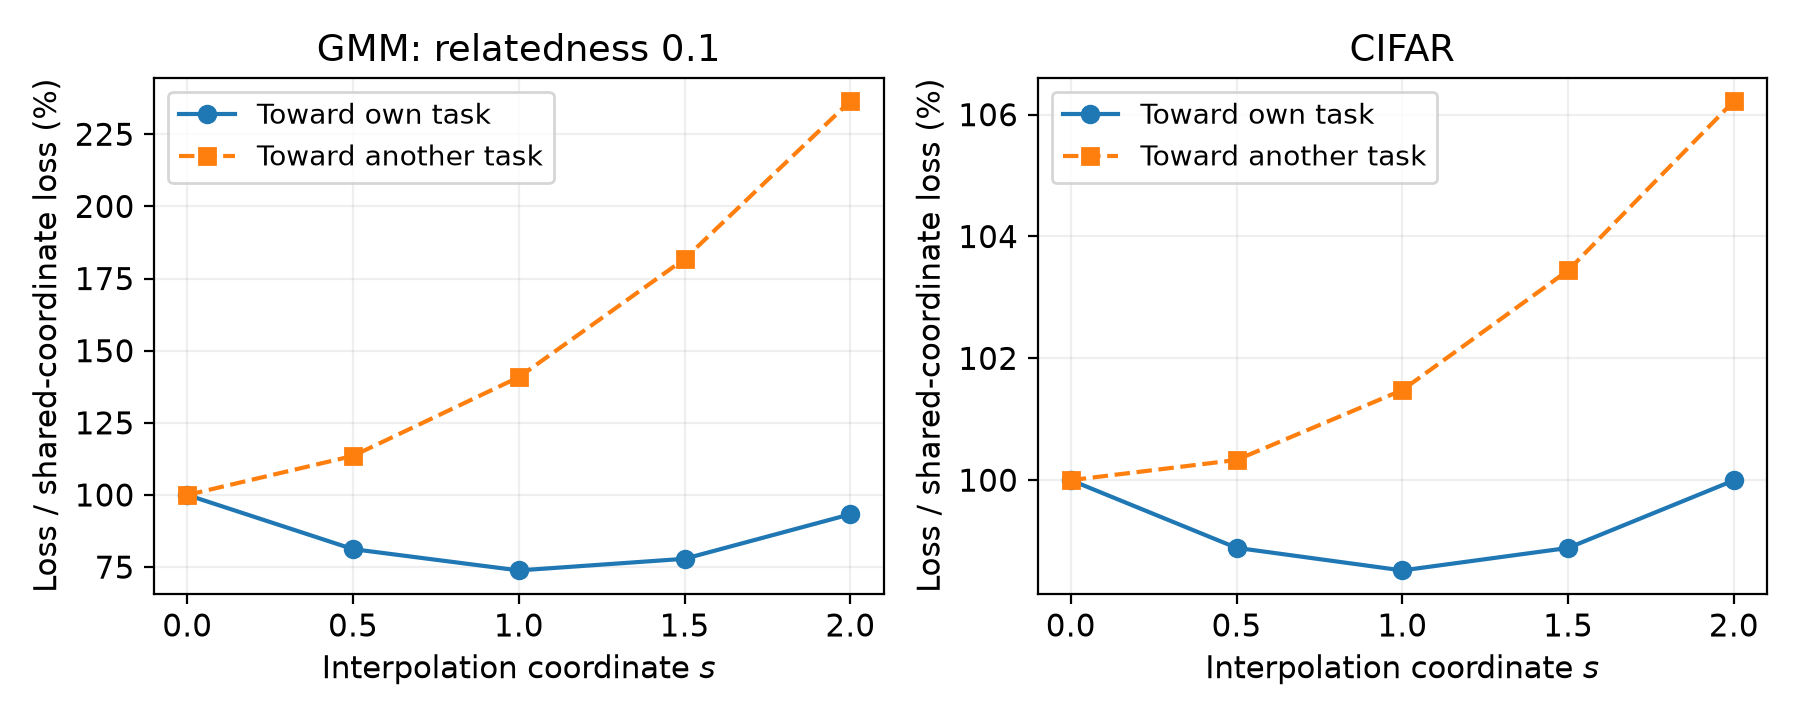
\includegraphics[width=.82\linewidth]{figures/profile_contrast.png}
\caption{\textbf{Task-coordinate interpolation.} The GMM and CIFAR panels use their respective model checkpoints. Losses are normalised by the shared-coordinate loss; own-task and wrong-task directions keep their diagnostic meanings. Their shapes do not replace the paired deployment-route comparisons.}
\label{fig:coord-profile}
\end{figure}

\FloatBarrier
\subsection{Complete factorial diagnostics}
The boundary experiment uses 64/16/64 train/validation/test semantic tasks, five model/data seeds, 8,000 training steps, linear transport and $\KT=0$. Source-task separation is controlled by $\alpha$ and relation heterogeneity by $\eta$ using the controlled construction described in the main experimental setup. The same latent tasks and perturbations are reused across neighbouring cells to support paired comparisons.

% Embedded GMM full matrices to avoid external-file dependency.
\begin{table*}[t]
\centering\scriptsize
\caption{Complete GMM factorial diagnostics. Top: correct-source advantage $G_{\rm source}=\mathrm{SW}_{wrong}-\mathrm{SW}_{correct}$. Middle: learned-coordinate task-ID accuracy. Bottom: held-out oracle affine relation $R^2$. Each cell averages five seeds; generation effects further average 64 held-out tasks per seed.}
\label{tab:gmm-full-matrices}
\vspace{2pt}\textbf{Correct-source advantage $G_{\rm source}$}\par\vspace{1pt}
\begin{tabular}{ccccccc}
\toprule $\alpha\backslash\eta$ & 0 & 0.1 & 0.25 & 0.5 & 1 & 2 \\ \midrule
0 & 0.000 & 0.000 & -0.000 & 0.000 & -0.000 & -0.002 \\
0.1 & 0.008 & 0.010 & 0.006 & 0.006 & 0.002 & 0.002 \\
0.25 & 0.093 & 0.102 & 0.098 & 0.066 & 0.038 & 0.023 \\
0.5 & 0.242 & 0.209 & 0.205 & 0.220 & 0.141 & 0.091 \\
0.75 & 0.387 & 0.391 & 0.370 & 0.321 & 0.256 & 0.142 \\
1 & 0.523 & 0.563 & 0.523 & 0.447 & 0.404 & 0.229 \\
1.5 & 0.693 & 0.736 & 0.715 & 0.661 & 0.567 & 0.427 \\
\bottomrule\end{tabular}\par\vspace{4pt}
\vspace{2pt}\textbf{Learned-coordinate task ID}\par\vspace{1pt}
\begin{tabular}{ccccccc}
\toprule $\alpha\backslash\eta$ & 0 & 0.1 & 0.25 & 0.5 & 1 & 2 \\ \midrule
0 & 0.014 & 0.016 & 0.016 & 0.020 & 0.018 & 0.013 \\
0.1 & 0.074 & 0.061 & 0.057 & 0.069 & 0.078 & 0.098 \\
0.25 & 0.338 & 0.340 & 0.316 & 0.282 & 0.324 & 0.349 \\
0.5 & 0.718 & 0.737 & 0.717 & 0.728 & 0.669 & 0.678 \\
0.75 & 0.866 & 0.861 & 0.849 & 0.845 & 0.825 & 0.791 \\
1 & 0.873 & 0.894 & 0.891 & 0.886 & 0.871 & 0.831 \\
1.5 & 0.928 & 0.920 & 0.925 & 0.920 & 0.908 & 0.882 \\
\bottomrule\end{tabular}\par\vspace{4pt}
\vspace{2pt}\textbf{Oracle affine relation $R^2$}\par\vspace{1pt}
\begin{tabular}{ccccccc}
\toprule $\alpha\backslash\eta$ & 0 & 0.1 & 0.25 & 0.5 & 1 & 2 \\ \midrule
0 & 1.000 & 0.849 & 0.509 & 0.227 & 0.067 & 0.007 \\
0.1 & 1.000 & 0.918 & 0.652 & 0.327 & 0.105 & 0.018 \\
0.25 & 1.000 & 0.975 & 0.861 & 0.609 & 0.277 & 0.077 \\
0.5 & 1.000 & 0.992 & 0.950 & 0.824 & 0.538 & 0.218 \\
0.75 & 1.000 & 0.995 & 0.971 & 0.892 & 0.672 & 0.333 \\
1 & 1.000 & 0.997 & 0.978 & 0.919 & 0.738 & 0.408 \\
1.5 & 1.000 & 0.997 & 0.984 & 0.939 & 0.794 & 0.487 \\
\bottomrule\end{tabular}\par\vspace{4pt}
\end{table*}

The full grid makes three distinctions visible. First, $G_{\rm source}$ is effectively zero at $\alpha=0$ even though a shared relation can still move the source distribution. Second, learned task discrimination increases much more slowly than Bayes identifiability around $\alpha=.1$--$.25$. Third, relation predictability falls with $\eta$ even when Bayes-ID is saturated. The mechanism analysis makes the second point sharper: the rank association with $G_{\rm source}$ is $\rho=.98$ for learned-ID versus $.69$ for Bayes-ID, and replacing Bayes-ID with learned-ID in the same interaction model increases cell-level fit from $R^2=.587$ to $.843$. These regressions are descriptive summaries of the factorial grid rather than causal estimates.

\begin{figure}[t]
\centering
\includegraphics[width=.72\linewidth]{results_file/fig_gain_vs_relation.png}
\caption{\textbf{Relation predictability is a separate boundary from task identifiability.} Each colour fixes source-task separation $\alpha$ while $\eta$ varies. The horizontal axis is the held-out $R^2$ of an affine map fitted to true training-task component means; it is therefore independent of Meta-Diff's learned coordinate. At $\alpha=1$, Bayes-ID remains 1.0 while relation $R^2$ falls from 1.000 to .408 and the correct-over-wrong SW advantage falls from .523 to .228. Over the full grid, $\rho(G_{\rm source},R^2_{\rm rel})=.53$.}
\label{fig:gmm-relation-app}
\end{figure}

\begin{figure*}[t]
\centering
\resizebox{.96\linewidth}{!}{\input{plots/gmm_full_grid_diagnostics.tex}}
\caption{\textbf{Full-grid GMM controls.} \emph{Left:} relation-only minus correct-source SW; positive values favour the source-conditioned route and stars mark hierarchical paired intervals excluding zero. \emph{Right:} true-source pairwise SW (in units of $10^{-3}$), an outcome-independent source-separation diagnostic. The source-conditioned route has a resolved advantage over relation-only in 33 of 42 cells; the full route tables also contain 34 resolved correct-versus-wrong cells, while source-reuse and oracle comparisons are not uniformly favourable.}
\label{fig:gmm-full-controls}
\end{figure*}


\subsection{Usable identity explains the source-specific gain}

The mechanism analysis compares intrinsic Bayes task identification with nearest-centroid identification in the learned source coordinate. Bayes-ID saturates rapidly, while learned-ID catches up only at much larger $\alpha$. Averaging across relation levels gives the following identity profile.

\begin{table}[h]
\centering\small
\caption{Intrinsic versus usable source-task identifiability. Chance is $1/64=.0156$. The collapse gap is Bayes-ID minus learned-ID.}
\begin{tabular}{cccc}
\toprule
$\alpha$ & Bayes-ID & learned-ID & Collapse gap\\
\midrule
0.00 & .016 & .016 & $-.001$\\
0.10 & .400 & .073 & .327\\
0.25 & .953 & .325 & \textbf{.628}\\
0.50 & 1.000 & .708 & .292\\
0.75 & 1.000 & .839 & .161\\
1.00 & 1.000 & .874 & .126\\
1.50 & 1.000 & .920 & .080\\
\bottomrule
\end{tabular}
\end{table}

The source-specific gain tracks usable learned identity more closely than the intrinsic ceiling. Across the 42 cells, $\rho(G_{\rm source},I_{\rm learned})=.98$ versus $\rho(G_{\rm source},I_{\rm Bayes})=.88$. Restricting to the 24 cells with Bayes-ID $>.99$ leaves $\rho(G_{\rm source},I_{\rm learned})=.97$. Descriptive cell-level regressions give:
The dedicated identity-pipeline retrieval uses an independently sampled retrieval protocol, so its learned-$z_S$ values below differ slightly from the phase-diagram learned-ID summary above; the qualitative ordering is unchanged.


\begin{table}[h]
\centering\small
\caption{Descriptive GMM regressions predicting $G_{\rm source}$. Intervals are those reported by the mechanism analysis.}
\begin{tabular}{lccc}
\toprule
Predictors & Fit $R^2$ & Key coefficient & 95\% CI\\
\midrule
Bayes-ID $+R^2_{\rm rel}+$ interaction & .587 & $I_{\rm Bayes}\!\times R^2_{\rm rel}=+.54$ & $[+.17,+.92]$\\
learned-ID $+R^2_{\rm rel}+$ interaction & \textbf{.843} & $I_{\rm learned}\!\times R^2_{\rm rel}=+.61$ & $[+.33,+.89]$\\
Bayes-ID $+$ learned-ID $+R^2_{\rm rel}$ & .814 & $I_{\rm learned}=+.73$ & $[+.55,+.91]$\\
& & $I_{\rm Bayes}=-.27$ & $[-.44,-.10]$\\
\bottomrule
\end{tabular}
\end{table}

The negative Bayes coefficient in the joint descriptive regression should not be interpreted causally; Bayes-ID and learned-ID share strong variation with $\alpha$. The robust point is that variation remaining in the learned coordinate continues to track the transfer benefit after intrinsic identification has saturated.

\subsection{Identity through the transport pipeline}

To locate where task information is lost, we retrieve the correct target task at successive stages of the pipeline. Transported-coordinate retrieval asks whether $\widetilde z_T=Az_S+b$ is closest to the correct held-out target coordinate. Raw $z_S\!\to z_T$ retrieval is a cross-domain baseline that omits transport.

\begin{table}[h]
\centering\small
\caption{Top-1 task identity through the GMM pipeline, averaged over relation levels and seeds. Chance is $1/64=.0156$.}
\begin{tabular}{ccccc}
\toprule
$\alpha$ & Bayes-ID & learned $z_S$ & transported $\widetilde z_T$ & raw $z_S\!\to z_T$\\
\midrule
0.00 & .016 & .015 & .013 & .016\\
0.10 & .400 & .071 & .019 & .015\\
0.25 & .953 & .323 & .089 & .023\\
0.50 & 1.000 & .691 & .169 & .039\\
0.75 & 1.000 & .831 & .258 & .074\\
1.00 & 1.000 & .883 & .315 & .109\\
1.50 & 1.000 & .920 & .341 & .148\\
\bottomrule
\end{tabular}
\end{table}

Identity is therefore compressed at both learned stages. Averaged over the grid, transported retrieval is $.172$, compared with $.061$ for raw cross-domain retrieval. The transport gain is resolved in every cell with $\alpha\geq.25$ ($+.112$ overall, paired seed-block interval $[+.106,+.116]$) and is absent at $\alpha=0$ and $.1$, where transported retrieval remains at chance. Across the 42 cells, $\rho(G_{\rm source},I_{\widetilde z_T})=.91$. The nearest-centroid margin for learned $z_S$ grows from $-.002$ at $\alpha=0$ to $+.060$ at $\alpha=1.5$, while the transported margin remains negative ($-.039$ to $-.079$), showing that transport improves task alignment without fully recovering the correct target coordinate.

\subsection{Source--target shift magnitude and transport headroom}

The phase diagram varies task identity and relation consistency. A separate sweep holds $\alpha=1,\eta=0$ fixed and changes only the magnitude of the shared transformation,
\[
T_\lambda(u)=u+\lambda(T_0(u)-u),
\qquad
\lambda\in\{0,.25,.5,1,2\}.
\]
This separates the value of choosing the correct source from the value of transporting that source.

\begin{table}[h]
\centering\small
\caption{GMM shift-magnitude sweep, averaged over tasks and five seeds. $G_{\rm source}=\mathrm{SW}_{\rm wrong}-\mathrm{SW}_{\rm correct}$; transport-over-reuse is $\mathrm{SW}_{\rm reuse}-\mathrm{SW}_{\rm correct}$.}
\begin{tabular}{ccccccc}
\toprule
$\lambda$ & Correct & Wrong & Relation-only & Source reuse & $G_{\rm source}$ & Transport over reuse\\
\midrule
0.00 & .759 & 1.241 & 1.062 & .783 & +.482 & +.024\\
0.25 & .765 & 1.252 & 1.048 & .828 & +.487 & +.063\\
0.50 & .802 & 1.315 & 1.115 & .905 & +.513 & +.102\\
1.00 & .835 & 1.355 & 1.157 & 1.066 & +.520 & +.231\\
2.00 & 1.037 & 1.667 & 1.443 & 1.577 & +.631 & +.541\\
\bottomrule
\end{tabular}
\end{table}

The source-specific gain remains large across the sweep because the semantic source task is identifiable even when $\lambda=0$. Transport-over-reuse behaves differently: it is an unresolved $.024$ at $\lambda=0$ and grows monotonically to $.541$ at $\lambda=2$. The independent model-free source--target SW headroom increases from approximately $.08$ to $1.59$ over the same sweep. This dissociation shows that source specificity and transport utility answer different questions: a correct source can matter even when there is almost nothing to transport.


\subsection{Historical representation-capacity and relatedness diagnostics}
The earlier MLP-era GMM suite is retained because it probes the representational ceiling, but it is not used as evidence for the final correct source $+$ transport route. Its aggregate summaries lack the paired task-level records needed to recover new confidence intervals.

\begin{table}[h]
\centering\small
\caption{Historical GMM representation-capacity diagnostic. The oracle fits an abundant-target coordinate; captured fraction is $(e_0-e_{\rm oracle})/(e_0-e_{\rm FT})$.}
\begin{tabular}{lrrrr}
\toprule
Configuration & No adapt. & Oracle & Conv. full FT & Captured\\
\midrule
$k=16$, 80k & .8821 & .6320 & .1276 & 33.2\%\\
$k=16$, 320k & .8741 & .5965 & .1508 & 38.4\%\\
$k=64$, 80k & .8868 & .5396 & .1267 & 45.7\%\\
$k=64$, 320k & .8779 & .4690 & .1565 & 56.7\%\\
\bottomrule
\end{tabular}
\end{table}

\begin{table}[h]
\centering\small
\caption{Historical GMM task-relatedness diagnostic at $k=16$, 80k steps. Larger template perturbations produce less related tasks.}
\begin{tabular}{lrrrr}
\toprule
Task family & No adapt. & Oracle & Full FT & Captured\\
\midrule
Perturbation .10 & .7513 & .3835 & .1179 & 58.1\%\\
Perturbation .25 & .8910 & .5583 & .1220 & 43.3\%\\
Perturbation .50 & .9516 & .6949 & .1359 & 31.5\%\\
Perturbation 1.00 & .9679 & .7808 & .1239 & 22.2\%\\
\bottomrule
\end{tabular}
\end{table}

These diagnostics support the intuitive claim that a compact shared representation has a higher ceiling when tasks are more closely related. Because the runs predate the final deployment protocol and report aggregate rather than paired route statistics, they are deliberately separated from the main claim.

\section{CIFAR-100: Full Controls and Ablations}
\label{app:cifar}

\subsection{Protocol}
Entire CIFAR-100 superclasses are assigned to train, validation or test so that close sibling classes do not cross the split. Twelve superclasses (60 fine classes) train the model, four superclasses (20 classes) are used for validation and hyperparameter selection, and four superclasses (20 classes) are held for final evaluation. A fixed permutation creates disjoint source and target pools: 300 source-support images, 50 source-query images, 20 reserved target-support images and 230 target-query images per class. Target transformations are Gaussian blur ($\sigma=1.0$), additive Gaussian noise (standard deviation $0.18$ on the normalised scale), and contrast reduction (factor $0.45$ toward the image mean), all at severity 3.

\subsection{Source specificity from zero to twenty targets}
This independent validation package adds mean-source and shuffled-source controls to the final-test comparison. 9 of nine main-relative source-control SW intervals favour correct source $+$ transport. Target-only comparisons favour transport at $K_T=1$; remain unresolved at $K_T=5,20$. Rows labelled source-initialised adaptation use the stated target-update budget; they do not implement direct target-free reuse.

\begin{table}[h]
\centering\small
\caption{CIFAR validation source-dependence sweep on the matched correct source $+$ transport evaluation: 180 total episodes, 60 per budget. Main transport and mean/shuffled/relation controls use $J=0$. Source-initialised adaptation starts at $z_S$ and uses target support; it is not strict reuse. SW is lower-is-better; paired $\Delta$ is comparator minus main, with episode-level 95\% half-widths and unrounded stars.}
\begin{tabular}{lccc}
\toprule
Route / comparison & $\KT=1$ & $\KT=5$ & $\KT=20$\\
\midrule
\shortstack[l]{correct source\\$+$ transport} & $0.2071\pm0.0192$ & $0.2077\pm0.0171$ & $0.2129\pm0.0193$\\
Source-init. adaptation & $0.2436\pm0.0197$ & $0.2351\pm0.0182$ & $0.2203\pm0.0220$\\
Target-only & $0.2255\pm0.0191$ & $0.2130\pm0.0191$ & $0.2087\pm0.0221$\\
Mean source & $0.2309\pm0.0201$ & $0.2347\pm0.0187$ & $0.2379\pm0.0204$\\
Shuffled source & $0.2417\pm0.0206$ & $0.2453\pm0.0191$ & $0.2469\pm0.0208$\\
Relation-only & $0.2413\pm0.0197$ & $0.2427\pm0.0185$ & $0.2476\pm0.0200$\\
\midrule
$\Delta$ Source-init. adaptation & $0.0366\pm0.0101\sigstar$ & $0.0274\pm0.0082\sigstar$ & $0.0074\pm0.0070\sigstar$\\
$\Delta$ Target-only & $0.0184\pm0.0076\sigstar$ & $0.0053\pm0.0055$ & $-0.0043\pm0.0084$\\
$\Delta$ Mean source & $0.0239\pm0.0067\sigstar$ & $0.0270\pm0.0075\sigstar$ & $0.0250\pm0.0074\sigstar$\\
$\Delta$ Shuffled source & $0.0347\pm0.0105\sigstar$ & $0.0376\pm0.0114\sigstar$ & $0.0340\pm0.0111\sigstar$\\
$\Delta$ Relation-only & $0.0342\pm0.0074\sigstar$ & $0.0350\pm0.0073\sigstar$ & $0.0347\pm0.0079\sigstar$\\
\bottomrule
\end{tabular}
\end{table}

\begin{figure}[t]
\centering
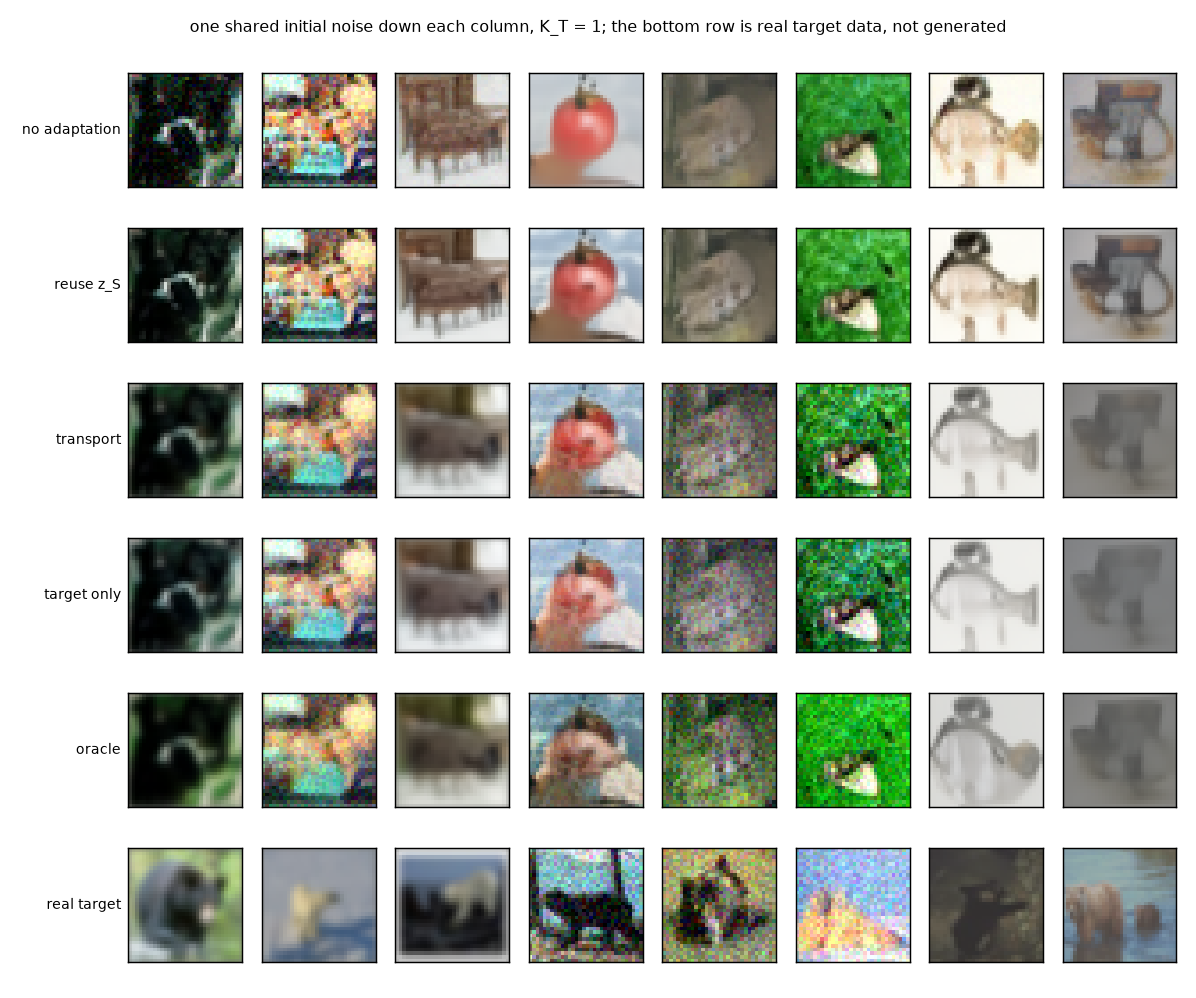
\includegraphics[width=.88\linewidth]{plots/strategy_grid.png}
\caption{CIFAR $K_T=1$ deployment grid from the 50k-step checkpoint. Exactly six rows show no adaptation, source-initialised target adaptation (the historical reuse-$z_S$ route), correct source $+$ transport with $J=0$, target-only, oracle, and real target. Generated rows share initial noise within each column; the real row is not generated. The transport-plus-refinement row is excluded.}
\label{fig:cifar-strategy-grid}
\end{figure}

The same final-test package gives energy MMD $2.3306, 2.3386, 2.4041$ for correct source $+$ transport, $3.4434, 2.5351, 2.4137$ for target-only, and $5.8971, 4.0219, 1.9086$ for full fine-tuning at $K_T=1,5,20$. Paired full-FT-minus-main differences are $3.5666\pm0.7496\sigstar$, $1.6833\pm0.6629\sigstar$, $-0.4955\pm0.3955\sigstar$. These comparisons favour transport at $K_T=1,5$; favour full fine-tuning at $K_T=20$. They use the same 60 matched episodes per budget and are not inferred from the SW intervals.


\subsection{Validation-frozen adaptation and target-time refinement}
\label{app:cifar-selection}

The full-fine-tuning settings were selected on validation tasks and frozen before correct source $+$ transport was evaluated on the final-test classes. They remain 25 steps at learning rate $10^{-5}$ for $\KT=1$, 25 at $10^{-4}$ for $\KT=5$, and 400 at $10^{-5}$ for $\KT=20$. No test result selects a new budget or model.

\begin{table}[h]
\centering\small
\caption{CIFAR validation-selected full-fine-tuning settings frozen before the matched final-test evaluation.}
\label{tab:cifar-ft-selection}
\begin{tabular}{ccc}
\toprule
Target budget & Full-FT steps & Learning rate\\
\midrule
$\KT=1$ & 25 & $10^{-5}$\\
$\KT=5$ & 25 & $10^{-4}$\\
$\KT=20$ & 400 & $10^{-5}$\\
\bottomrule
\end{tabular}
\end{table}

The five-budget A3 refinement experiment compares matched on/off conditions on the 50k-step \texttt{cifar\_ds3} checkpoint. It uses 300 validation episodes (60 at each $K_T$), matched target support/query sets and paired refinement/generation noise. The metric is transformation-statistic distance. Gain is transport alone minus transport plus 25 refinement steps; positive favours refinement. This separate diagnostic is not pooled with final-test SW or MMD.

\begin{table}[h]
\centering\small
\caption{Matched refinement ablation on the correct source $+$ transport checkpoint. $J=0$ remains the main route; the ablation uses $J=25$, learning rate $0.01$ and the same prior/noise budget. Half-widths are $1.96\,\mathrm{SE}$ over 60 paired class--transformation episodes per budget; stars use unrounded gain intervals.}
\label{tab:cifar-refinement}
\begin{tabular}{lccccc}
\toprule
 & $\KT=1$ & $\KT=2$ & $\KT=5$ & $\KT=10$ & $\KT=20$\\
\midrule
Refinement gain & $-0.0244\sigstar$ & $-0.0071$ & $-0.0267$ & $+0.0144$ & $-0.0065$\\
95\% half-width & $0.0136$ & $0.0169$ & $0.0320$ & $0.0348$ & $0.0434$\\
\bottomrule
\end{tabular}
\end{table}

The gain interval is negative at $K_T=1$: refinement worsens transformation-statistic distance in that comparison. The other four intervals contain zero; this establishes neither equivalence nor universal absence of benefit. The separate source-initialised target-adaptation baseline starts from $z_S$ and uses target evidence. Its behaviour cannot be inferred from the post-transport gains in this table, and it must not be called strict direct reuse.

\subsection{Source budget and conditioning generality}
The source-budget sweep shows small changes between $M_S=16$ and 300, but not exact equivalence: the paired SW difference at $M_S=64$ relative to 16 is $-0.00287\pm0.00236\sigstar$. Other measured increments relative to 16 have intervals containing zero; no $M_S<16$ was tested. The model was trained with $M_S=64$ and evaluated at $K_T=1$ with nested source prefixes and matched query/noise. Proposition~\ref{prop:source-concentration} concerns coordinate estimation error, not equivalence of generated SW at all source sizes.

In the independent 180-episode FiLM validation package, SW for correct source $+$ transport is $0.1973, 0.1942, 0.1987$ and fine-class consistency is $0.1306, 0.1278, 0.1311$ at $K_T=1,5,20$. Mean-source SW is $0.2417, 0.2441, 0.2462$, shuffled-source $0.2567, 0.2578, 0.2616$, and relation-only $0.2366, 0.2373, 0.2414$. All 9/9 SW and 9/9 semantic main-relative intervals favour the correct source. Paired consistency gains are $0.0740\pm0.0234\sigstar$, $0.0786\pm0.0253\sigstar$, $0.0780\pm0.0245\sigstar$ against mean source, $0.0835\pm0.0233\sigstar$, $0.0799\pm0.0258\sigstar$, $0.0835\pm0.0255\sigstar$ against shuffled source, and $0.0757\pm0.0218\sigstar$, $0.0773\pm0.0238\sigstar$, $0.0773\pm0.0220\sigstar$ against relation-only. These source controls do not test the full FiLM target-only/full-FT crossover.

\begin{table}[h]
\centering\small
\caption{Three independent matched CIFAR SW packages. Upper block: correct source $+$ transport with two conditioning architectures. Lower blocks: transport-structure ablations, with direct $J=0$ generation in both compared arms. Pairing is within block only; all intervals are over validation episodes at one training seed per arm.}
\begin{tabular}{lccc}
\toprule
Configuration / comparison & $\KT=1$ & $\KT=5$ & $\KT=20$\\
\midrule
\shortstack[l]{Basis: correct source\\$+$ transport} & $0.2067\pm0.0192$ & $0.2090\pm0.0177$ & $0.2136\pm0.0196$\\
\shortstack[l]{FiLM: correct source\\$+$ transport} & $0.1973\pm0.0206$ & $0.1942\pm0.0164$ & $0.1987\pm0.0193$\\
FiLM $-$ basis & $-0.0094\pm0.0099$ & $-0.0148\pm0.0107\sigstar$ & $-0.0149\pm0.0107\sigstar$\\
\midrule
Basis residual MLP & $0.2102\pm0.0190$ & $0.2109\pm0.0165$ & $0.2138\pm0.0193$\\
Basis linear & $0.2124\pm0.0211$ & $0.2113\pm0.0183$ & $0.2174\pm0.0210$\\
Linear $-$ MLP & $0.0022\pm0.0049$ & $0.0004\pm0.0048$ & $0.0036\pm0.0050$\\
\midrule
FiLM nonlinear & $0.2066\pm0.0224$ & $0.2054\pm0.0185$ & $0.2074\pm0.0214$\\
FiLM linear & $0.1973\pm0.0206$ & $0.1942\pm0.0164$ & $0.1987\pm0.0193$\\
Nonlinear $-$ linear & $0.0093\pm0.0037\sigstar$ & $0.0112\pm0.0040\sigstar$ & $0.0087\pm0.0042\sigstar$\\
\bottomrule
\end{tabular}
\end{table}

In the retained FiLM transport-structure ablation, nonlinear-minus-linear MMD differences are $0.2479\pm0.1658\sigstar$, $0.2810\pm0.1588\sigstar$, $0.1958\pm0.1640\sigstar$, all favouring linear transport. They are paired effects, not raw MMD values. The matched conditioning comparison favours FiLM at $K_T=5,20$, with the other budgets unresolved. The basis and FiLM conditioning counts remain 55,344 and 118,784 (46.6\% ratio). Their evaluated score paths have 27,798,195 and 27,916,979 parameters, respectively; the shared transport module adds the same 352 registered parameters (304 active). No latency, FLOP or memory conclusion is inferred.

\subsection{Meta-training-task scarcity}
Both task-scarcity arms use correct source $+$ transport and $J=0$, with 50\% (30/60 classes, all 12 superclasses) and 25\% training subsets. At 50\%, FiLM-minus-basis SW effects are $-0.0098\pm0.0119$, $-0.0102\pm0.0128$, $-0.0104\pm0.0135$; all three intervals contain zero. FiLM-minus-basis MMD effects are $-0.3484\pm0.3090\sigstar$, $-0.5448\pm0.3468\sigstar$, $-0.5468\pm0.4052\sigstar$, and superclass-consistency effects are $0.0363\pm0.0211\sigstar$, $0.0380\pm0.0232\sigstar$, $0.0335\pm0.0225\sigstar$. The MMD and consistency contrasts favour FiLM. At 25\%, SW effects are $0.0027\pm0.0076$, $0.0007\pm0.0080$, $-0.0003\pm0.0076$, all unresolved. These SW intervals do not establish an architecture ranking or a ranking reversal. Each arm has one training seed; episode intervals do not cover training-seed uncertainty.

\subsection{Coordinate retrieval and direct-target diagnostics}
The frozen 50k FiLM model was probed to separate coordinate inference from generation. With 20 held-out candidate classes, correct-source transport achieves L2 target-coordinate retrieval of 62.5\%, 59.5\%, and 49.0\% for blur, noise, and contrast, respectively; raw $z_S$ achieves 17.25\%, 26.5\%, and 14.0\%, and wrong-source transport achieves 1.25\%, .75\%, and 2.25\%. Support-resampling intervals for all main-minus-raw and main-minus-wrong L2 differences exclude zero.

Bypassing transport does not guarantee semantic generation. Direct target coordinates estimated from 200 target images give held-out generated identity of 3.59\% (blur), 3.85\% (noise), and 2.71\% (contrast), compared with real-query identity of 51.2\%, 34.5\%, and 70.9\%. Diffusion-time probes nevertheless show that correct target coordinates lower denoising MSE in most held-out timestep bins, including all three highest-noise bins. The evidence therefore supports coordinate use without implying that coordinate use alone guarantees class-correct generation.

\section{Office-Home: Full Natural-Domain Stress Test}
\label{app:office}

\subsection{Protocol and evaluator audit}
The corrective Office-Home experiment uses the Product$\rightarrow$Clipart relation, 45/10/10 train/validation/test semantic classes, $64\times64$ images, FiLM conditioning, linear transport and the effective-batch-64 training run. Ten held-out classes are the independent inference units; eight generation repeats and wrong-source assignments are averaged within class before the 10,000-draw class bootstrap.

\begin{table}[h]
\centering\small
\caption{Office-Home real-image evaluator audit.}
\begin{tabular}{lc}
\toprule
Check & Result\\
\midrule
CLIP top-1, Product / Clipart & 89.03\% / 65.96\%\\
Test classes with Clipart top-1 $\geq30\%$ & 10/10\\
DINOv2 held-out domain accuracy & 98.30\%\\
Same-class centroid top-1 / median rank & 100.0\% / 1\\
Same-minus-different centroid cosine gap & .5077\\
\bottomrule
\end{tabular}
\end{table}


\subsection{Validation-only checkpoint and adaptation selection}

All Office-Home model and adapting-baseline choices were fixed on the ten validation classes before the outer test. Validation DINO-SW decreased monotonically across the saved checkpoint sequence, and the 50,000-step checkpoint was selected for the final route comparisons.

\begin{table}[h]
\centering\small
\caption{Office-Home validation-only selection record. The upper block reports the main-route checkpoint trajectory. The lower block reports the budget-specific target-only and full-fine-tuning settings subsequently frozen for final testing. These validation values are not pooled with test results.}
\label{tab:office-selection}
\begin{tabular}{rc}
\toprule
Checkpoint step & Main $\KT=0$ DINO-SW\\
\midrule
20,000 & .040525\\
25,000 & .039609\\
30,000 & .038712\\
35,000 & .038019\\
40,000 & .037572\\
45,000 & .037351\\
50,000 & .037283\\
\bottomrule
\end{tabular}

\vspace{4pt}
\begin{tabular}{crrrrrr}
\toprule
$\KT$ & Target steps & Target lr & Target val SW & Full-FT steps & Full-FT lr & Full-FT val SW\\
\midrule
1 & 5 & .030 & .037660 & 100 & $3{\times}10^{-5}$ & .036521\\
5 & 5 & .010 & .038021 & 400 & $3{\times}10^{-5}$ & .034206\\
10 & 5 & .030 & .037397 & 400 & $3{\times}10^{-5}$ & .032314\\
\bottomrule
\end{tabular}
\end{table}

A separate validation-only zero-target code-path check gave DINO-SW .037239 for correct-source transport, .038168 for wrong-source transport, .037950 for relation-only prediction and .040021 for source reuse. These values are selection/audit evidence only; all superiority claims in the paper use the held-out test route matrices below.

\subsection{Zero-target and target-budget results}
\begin{table}[h]
\centering\small
\caption{Office-Home $\KT=0$ route matrix. Distance metrics are lower-is-better; requested-class and Clipart fractions are higher-is-better.}
\begin{tabular}{lrrrr}
\toprule
Route & DINO-SW & MMD & Object ID (\%) & Clipart (\%)\\
\midrule
Correct $+$ transport & .038969 & .407846 & 1.67 & 86.50\\
Wrong $+$ transport & .039394 & .419016 & 1.44 & 86.27\\
Relation-only & .039251 & .415280 & 1.37 & 86.71\\
Source reuse & .041641 & .457524 & 1.18 & 63.80\\
\bottomrule
\end{tabular}
\end{table}

The paired SW gain over wrong-source transport is $.000425$ $[.000213,.000643]$; over relation-only it is $.000282$ $[.000109,.000456]$; over source reuse it is $.002673$ $[.002270,.003036]$. Requested-class differences from wrong and relation-only are unresolved. Thus the zero-target claim is distributional/domain alignment rather than reliable semantic transfer.

\begin{table}[h]
\centering\small
\caption{Office-Home target-budget summary. Correct-source transport uses no target images and is therefore constant across budgets.}
\begin{tabular}{lcccc}
\toprule
$\KT$ & Route & DINO-SW & Object ID (\%) & Clipart (\%)\\
\midrule
1 & Correct $+$ transport & .038969 & 1.67 & 86.50\\
1 & Target-only & .040346 & 2.23 & 75.73\\
1 & Full FT & .039336 & 5.33 & 87.49\\
\midrule
5 & Correct $+$ transport & .038969 & 1.67 & 86.50\\
5 & Target-only & .039031 & 1.81 & 81.22\\
5 & Full FT & .034550 & 12.55 & 83.11\\
\midrule
10 & Correct $+$ transport & .038969 & 1.67 & 86.50\\
10 & Target-only & .039001 & 1.61 & 82.79\\
10 & Full FT & .033859 & 12.01 & 83.82\\
\bottomrule
\end{tabular}
\end{table}

At $\KT=1$, transport improves DINO-SW over target-only with paired difference $.001377$ $[.000568,.002311]$; its SW comparison with full fine-tuning is unresolved, although its MMD is better. At $\KT=5$ and $10$, full fine-tuning is significantly better in SW, MMD and requested-object accuracy.

\begin{figure}[t]
\centering
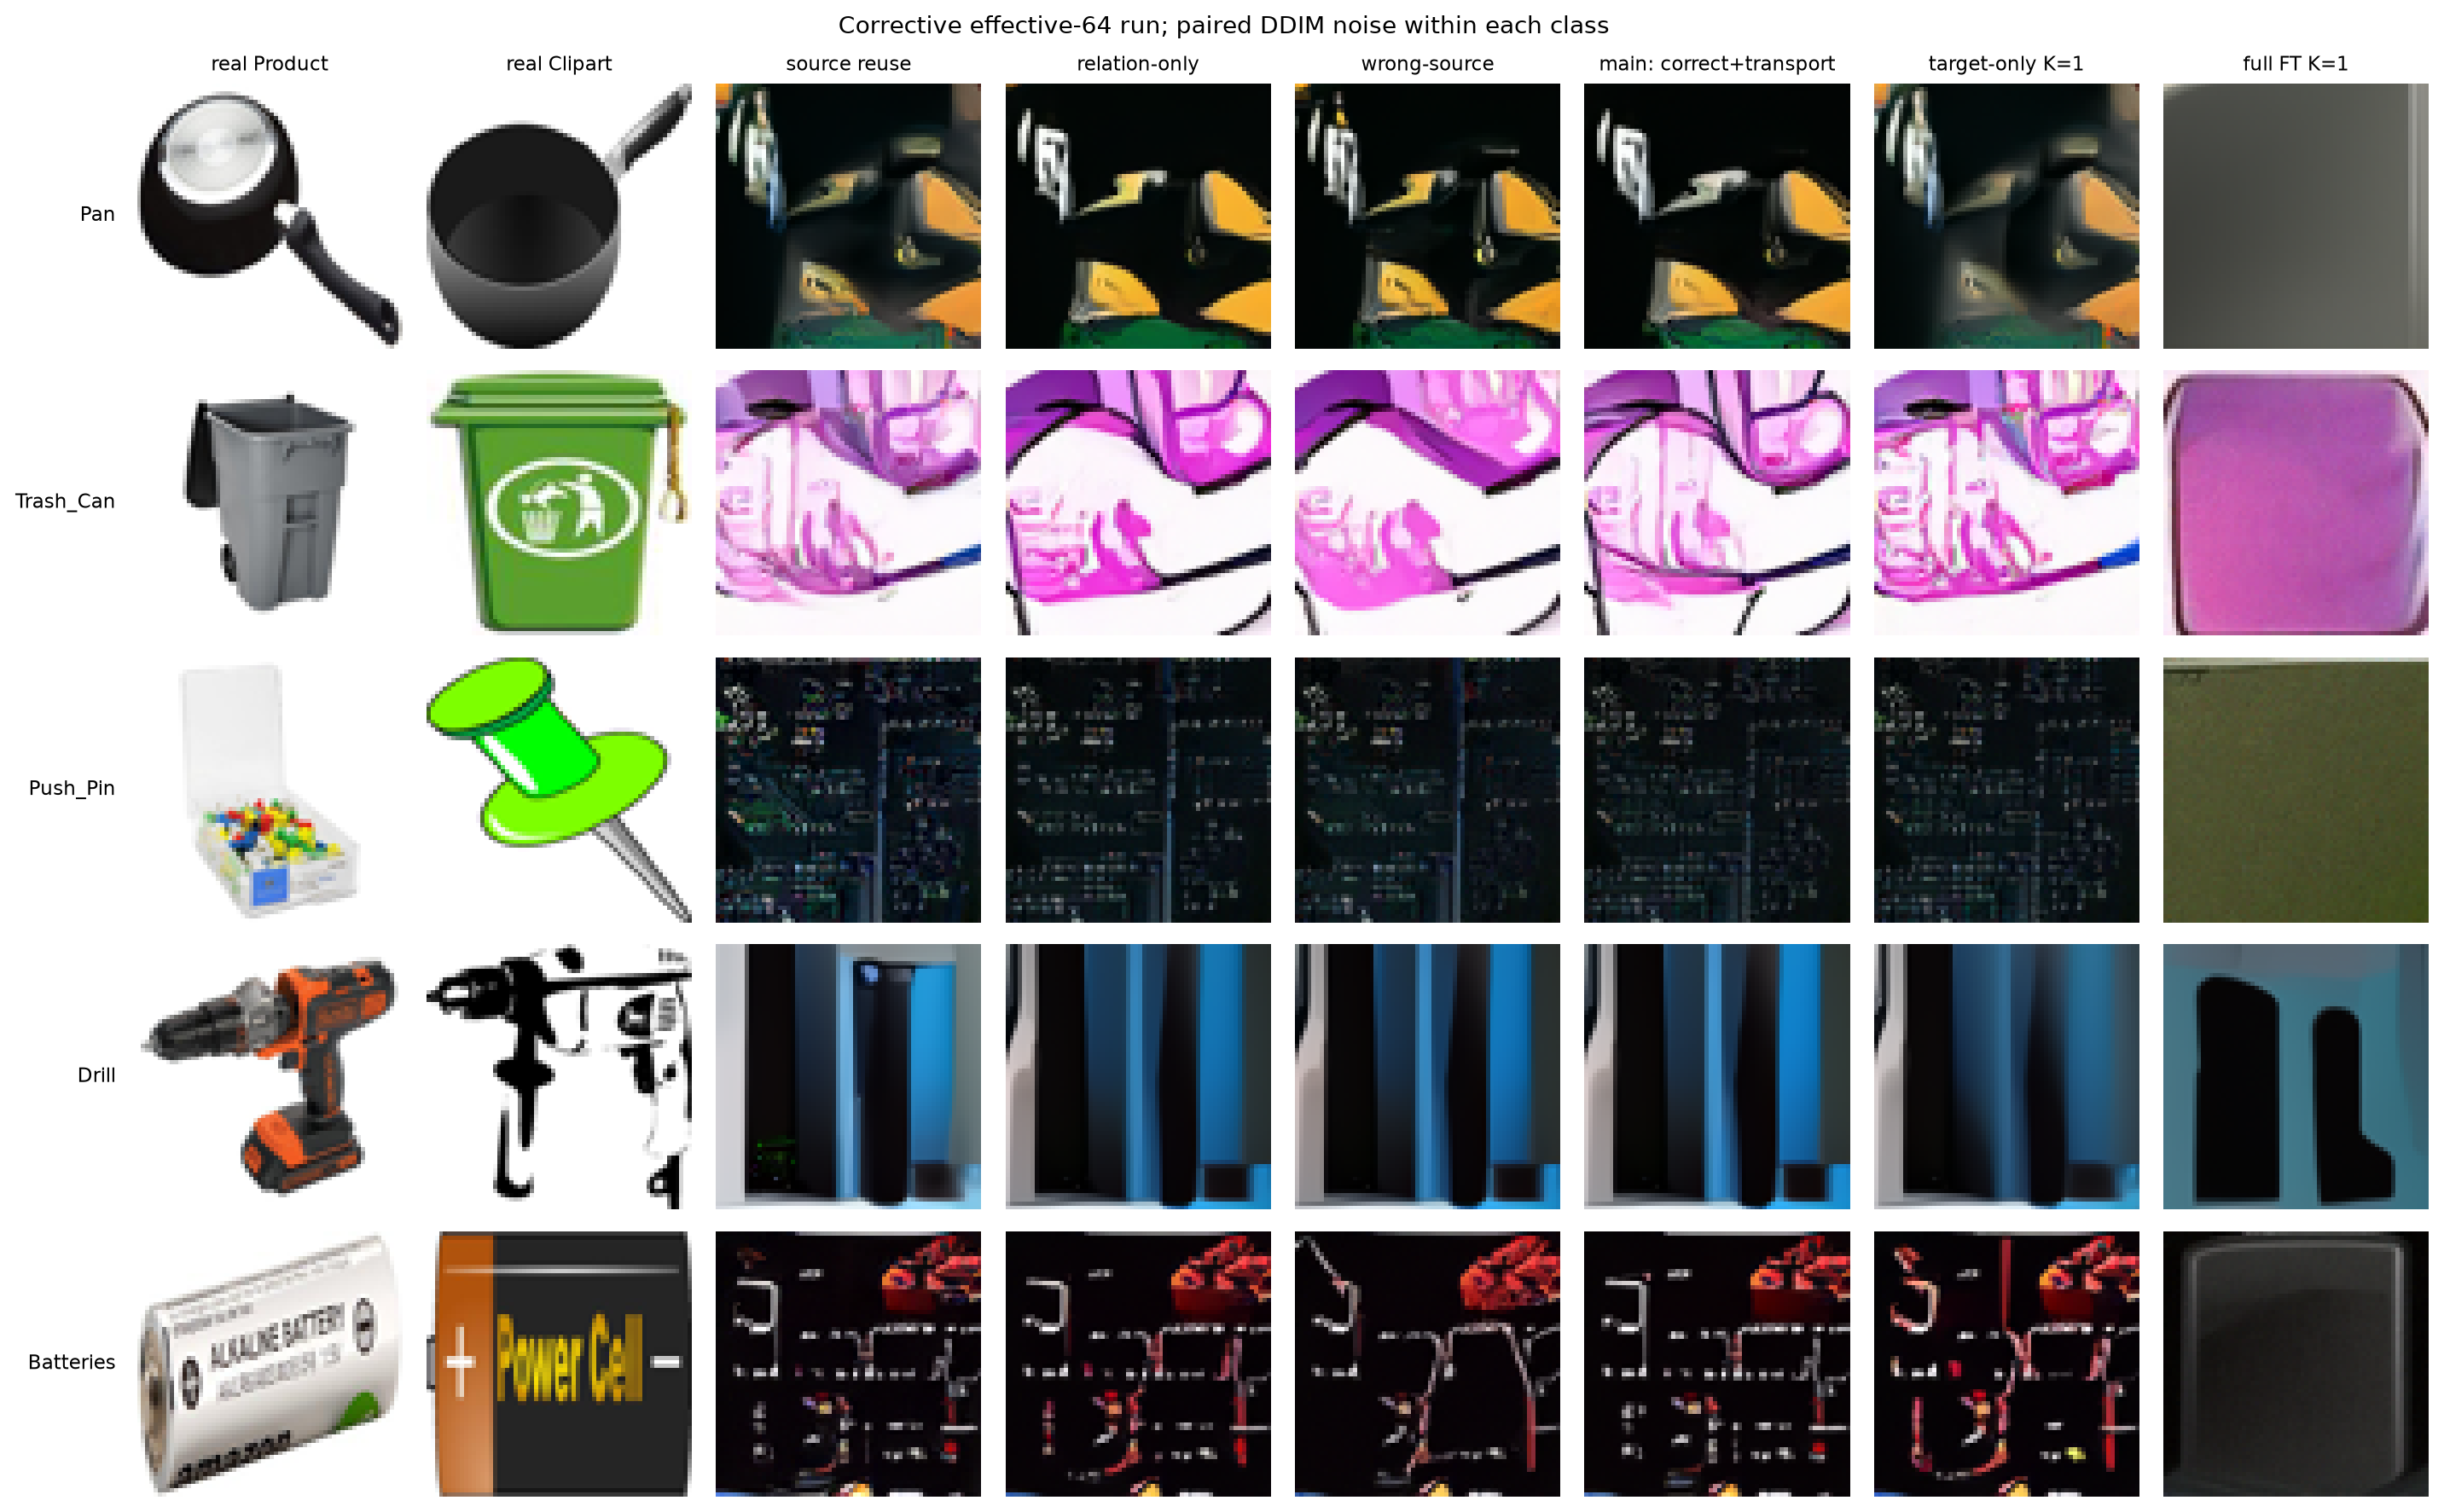
\includegraphics[width=.98\linewidth]{plots/O-F1_generation_grid.png}
\caption{Office-Home generation grid. Columns are held-out classes. Rows contain real Product, real Clipart, source reuse, relation-only, wrong-source transport, correct-source transport, one-shot target-only and one-shot full fine-tuning. Generated routes share DDIM noise within class.}
\end{figure}

\subsection{Localising the semantic bottleneck}
Four frozen-checkpoint diagnostics probe where object identity is lost.

\begin{table}[h]
\centering\small
\caption{Office-Home target-coordinate retrieval on ten held-out classes.}
\begin{tabular}{lrrrr}
\toprule
Query route & L2 top-1 & Cosine top-1 & L2 margin & Cosine margin\\
\midrule
Raw $z_S$ & 12.0\% & 26.5\% & -.0500 & -.1749\\
Correct source $+$ transport & 42.0\% & 44.5\% & -.0153 & -.0620\\
Wrong-source transport & 20.0\% & 19.0\% & -.0897 & -.2654\\
Relation-only & 10.0\% & 10.0\% & -.0545 & -.1510\\
\bottomrule
\end{tabular}
\end{table}

Correct transport significantly improves L2 retrieval over raw $z_S$ and both L2/cosine retrieval over relation-only, but the correct-versus-wrong transport class intervals include zero. This is partial coordinate alignment rather than a resolved source-specific retrieval result.

\begin{table}[h]
\centering\small
\caption{Office-Home direct-$z_T$ generation using abundant non-query Clipart support.}
\begin{tabular}{lrrrrr}
\toprule
Group & Generated ID & Real ID & DINO-SW & DINO-MMD & Clipart\\
\midrule
Seen (45 classes) & 2.38\% & 50.33\% & .03679 & .35175 & 87.34\%\\
Held-out (10 classes) & 1.56\% & 52.00\% & .03902 & .40642 & 88.33\%\\
\bottomrule
\end{tabular}
\end{table}

Bypassing transport therefore does not restore object identity. The held-out-minus-seen generated-identity contrast is $-.82$ percentage points with 95\% interval $[-2.45,.76]$.

The diffusion-time probe replaces the correct target coordinate with a cyclic wrong-class coordinate while holding query image, noise and timestep fixed. On seen classes, wrong-minus-correct MSE is positive in all five timestep bins; on held-out classes it is positive with intervals excluding zero in three of five bins. The highest-noise differences are only $5.5\times10^{-5}$ (seen) and $1.7\times10^{-5}$ (held-out), showing weak but nonzero coordinate use.

Finally, an explicit 16-D learned class embedding provides a matched capacity control for the FiLM interface. On seen Clipart classes, generated identity rises from 2.38\% with direct learned $z_T$ to 6.90\%, a paired gain of 4.51 percentage points $[2.85,6.37]$; DINO-SW and MMD also improve. Because 6.90\% remains far below the 50.33\% real-image calibration, the control demonstrates partial semantic conditioning capacity rather than a complete solution.

\section{Clinical and External-Domain Stress Tests}
\label{app:clinical}
These studies are retained for transparency and boundary analysis. They are not used as positive evidence for clinical or demographic source-specific transfer.

\subsection{ChestX-ray14 age-group transfer}
Tasks are single-positive thoracic findings, source ages are 45--60, and target ages are 0--30, 30--45 and 60--75. The fixed 4/2/3 finding split uses whole-patient allocation. Evaluation covers three held-out findings, three age relations and four resamples, with $\MS=64$.

\begin{table}[h]
\centering\scriptsize
\caption{ChestX-ray14 SW route means. Lower is better. The independently reported wrong-minus-correct paired interval at $\KT=1$ is $7.7\times10^{-6}\pm2.3\times10^{-5}$; other displayed route differences lack paired covariance information.}
\resizebox{\linewidth}{!}{%
\begin{tabular}{lccccc}
\toprule
Method & $\KT=1$ & $2$ & $5$ & $10$ & $20$\\
\midrule
No adaptation & .3696 & .3696 & .3696 & .3696 & .3696\\
Target-only & .1397 & .1406 & .1398 & .1405 & .1408\\
Relation-only & .3680 & .3680 & .3680 & .3680 & .3680\\
Wrong-source transport & .1407 & .1407 & .1407 & .1407 & .1407\\
Correct source $+$ transport & .1407 & .1407 & .1407 & .1407 & .1407\\
Full fine-tuning & .2981 & .2802 & .2304 & .1800 & .1591\\
\bottomrule
\end{tabular}}
\end{table}

Correct-source transport reaches the broad target-image distribution far better than no adaptation or relation-only, but wrong-source transport has the same rounded mean and the available paired correct-versus-wrong contrast is unresolved. The finding classifier has only 12.1\% accuracy and an abundant-target age diagnostic has slope $.039\pm.064$, so neither image distance nor predictor output validates the requested age/finding identity. This branch therefore establishes broad distribution matching, not source-specific demographic transfer.

\subsection{Fitzpatrick17k disease and pathology-family transfer}
All 16,577 official rows were recovered from the SFU renamed archive, matched to the official CSV by MD5, and filtered through the published cleaned allow-list. The retained set contains 11,394 images, of which 11,098 have Fitzpatrick type I--VI. The disease-level split is 8/4/4 train/validation/test diseases. Pathology-family follow-ups use six test families for I--III$\rightarrow$IV--VI and five for I--III$\rightarrow$V--VI.

\begin{table}[h]
\centering\scriptsize
\caption{Fitzpatrick zero-target route means. Invalidated phenotype/semantic instruments are omitted here; statistic distance, SW and energy MMD are lower-is-better.}
\resizebox{\linewidth}{!}{%
\begin{tabular}{llrrr}
\toprule
Protocol & Route & Statistic & SW & MMD\\
\midrule
Disease IV--VI & Source reuse & 2.5248 & .3642 & 7.1765\\
& Wrong disease, same family & 2.5020 & .3638 & 7.1466\\
& Wrong disease, different family & 2.5025 & .3639 & 7.1444\\
& Correct source $+$ transport & 2.5030 & .3638 & 7.1429\\
\midrule
Family IV--VI & Source reuse & 1.7452 & .3081 & 5.7946\\
& Wrong-family transport & 1.7185 & .3064 & 5.7468\\
& Correct source $+$ transport & 1.7188 & .3063 & 5.7436\\
\bottomrule
\end{tabular}}
\end{table}

Disease-level correct-source and wrong-source routes are indistinguishable on the valid distributional metrics. The same conclusion holds at pathology-family resolution: correct source has no resolved advantage over wrong-family transport. The stronger I--III$\rightarrow$V--VI follow-up also fails to recover source specificity; the wrong-task-minus-correct paired effects are $-.00068\pm.00273$ for statistic distance, $-.00003\pm.00134$ for SW and $-.00107\pm.03907$ for MMD.

The interpretation is further constrained by the evaluators. The pathology-family semantic gate fails on every outer fold in the stronger split, and an exploratory phenotype audit finds real-target recall of 0\% for IV--VI and 0--6.3\% for V--VI despite high aggregate accuracy. A source-only disease-separability analysis reports $\rho=-.775$ over four diseases, but three of the four semantic effects are exactly zero and only 6,793/10,000 bootstrap draws have defined rank variance. We therefore do not use task separability as the central explanation for the Fitzpatrick result. Downstream demographic augmentation was not run because the pre-specified positive family-semantic gate was not met.

\subsection{CRC histology preflight}
CRC uses NCT-CRC-HE-100K as source and CRC-VAL-HE-7K as external target over nine tissue classes and three outer folds. A prespecified gate required both a valid tissue evaluator and sufficient source--target domain separation before any Meta-Diff training.

\begin{table}[h]
\centering\small
\caption{CRC real-image preflight and stopping decision.}
\begin{tabular}{lc}
\toprule
Check & Result\\
\midrule
Target tissue balanced accuracy & 88.25\%\\
Minimum target tissue recall & 60.57\%\\
Domain balanced accuracy, fold 1 & 59.01\%\\
Domain balanced accuracy, fold 2 & 58.24\%\\
Domain balanced accuracy, fold 3 & 57.00\%\\
Same-tissue centroid retrieval & 100\% top-1 in each fold\\
Diffusion training / generation & Not run: structural gate failed\\
\bottomrule
\end{tabular}
\end{table}

The tissue evaluator and cross-domain tissue alignment pass, but all three domain-separation folds fall below the locked 70\% threshold. No CRC generation result exists. The stop therefore concerns benchmark suitability under the frozen representation and provides no evidence for or against Meta-Diff generation performance.

\section{Implementation and Reproducibility}
The CIFAR score model uses a 128-base-channel U-Net and $k=16$ coordinates; its encoder has approximately 0.33M parameters. The basis contributes 55,344 conditioning parameters. The actual three-relation linear transport is $Az_S+b_c$: $16^2+3\times16=304$ active parameters. Its saved module has 352 registered parameters because a 48-value compatibility embedding is not used by its forward map. A single-relation affine map has $16^2+16=272$ parameters. Every headline CIFAR route directly decodes the predicted coordinate at all $K_T$, without target input, coordinate refinement or backbone update. Office-Home retains its separate 64-base-channel, $64\times64$ FiLM model, DDIM-50 and no-refinement headline protocol.

Semantic splits are fixed and target support/query images are disjoint. Within each CIFAR package, routes share the task, support/query episode and generation noise; the episode-level $1.96\,\mathrm{SE}$ intervals and their nested class dependence are stated explicitly. Independent conditioning packages are not pooled. Validation-selected full-FT budgets are frozen before matched final-test evaluation, and no test score selects a new model, budget or subset. Other benchmarks retain their own frozen protocols and statistical units.

The paper distinguishes final-model interventions from historical evidence. The GMM calibration table, two-panel interpolation profile and main-text own/mean/shuffled/zero generation grid use their separately identified checkpoints; these diagnose coordinates, not deployment superiority. Historical GMM capacity/relatedness aggregates remain accurately labelled in the appendix, and transport-structure ablations compare MLP and linear maps. The refinement table reports matched on/off measurements on the correct source $+$ transport checkpoint. Frozen-coordinate and direct-target semantic probes are reported as independent diagnostics.